%%%%%%%%%%%%%%%%%%%%%%%%%%%%%%%%%%%%%%%%%%%%%%%%%%%%%%%%%%%%%%%%%%%%%%%%%%%
%The discovery of \bbonu\ would represent a substantial breakthrough in particle physics. A single, unequivocal observation of the decay would prove the Majorana nature of neutrinos and the violation of lepton number. Alas, that is not, by any means, an easy task. The design of a detector capable of identifying efficiently and unambiguously such a rare signal represents a major experimental challenge.

Given the sensitivity to $T_{1/2}^{0\nu}$ already achieved, the first ingredient required for the next generation of \bbonu\ experiment is a 
%To start with, one needs a
 large mass of a suitable (and always scarce) \bb\ isotope in order to probe in a reasonable time the extremely long lifetimes expected. 
% For instance, for a Majorana neutrino mass of 18 meV, corresponding to the lowest possible \mbb\ value in the inverted ordering scenario (see fig.~\ref{fig:mbetabetavsmlight}), it can be estimated using eq.~(\ref{eq:Tonu}) and a sound assumption for the NMEs that half-lives in the range of $10^{27}$--$10^{28}$ years must be explored (\textit{i.e.}, at least 17 orders of magnitude longer than the age of the universe!). 
 %A better sense of what such extremely long half-lives mean can be grasped with a 
 %
 This can be easily illustrated with a simple calculation. Consider the radioactive decay law in the approximation $T_{1/2}\gg t$, where $t$ is the exposure time; in that case, the expected number of \bbonu\ events is given by
%
\begin{equation}
N_{\bbonu} = \log2 \cdot \frac{\Mbb\cdot N_{A}}{W_{\beta\beta}} \cdot \varepsilon \cdot \frac{t}{T_{1/2}^{0\nu}}, 
\label{eq:Nbb}
\end{equation}
%
where \Mbb\ is the mass of the \bb\ emitting isotope, $N_{A}$ is the Avogadro constant, $W_{\beta\beta}$ is the molar mass of the \bb\ isotope, and $\varepsilon$ is the signal detection efficiency.

Take \Xe{136} as an example, and assume that one aims to achieve a sensitivity 
$T_{1/2}^{0\nu}\sim 10^{27}$ years (e.g, one order of magnitude better than current limits). In the absence of backgrounds, the observation of a single event implies a discovery. Solving eq.~\ref{eq:Nbb} for $ N_{\bbonu}=1$, $T_{1/2}^{0\nu} = 10^{27}$ years, $\epsilon = 1$ (perfect detector) and $t = 1$ year, yields  $\Mbb \sim 330$ kg. Considering a realistic efficiency $\epsilon \sim 0.3--0.6$, would result in an isotope mass in the range of one ton, just to observe one event per year.  

%It follows from eq.~(\ref{eq:Nbb}) that, in order to observe (assuming perfect detection efficiency and no disturbing background) as little as one decay per year and assuming a Majorana neutrino mass of 18 meV ($T_{1/2}^{0\nu}\sim 10^{27}$--$10^{28}$ years), masses of \bb\ isotope of the order of one tonne are needed.

On the other hand, in the presence of backgrounds, the observation of a single event is not enough to establish a discovery. Imagine now that our putative \Xe{136} experiment predicts a background of one event per year. Since the process is Poisson distributed, the probability of observing, say, 9 events when 1 is expected is $sim 10^{-6}$. Observing 9 events would therefore establish a discovery at roughly 5$\sigma$, while observing 5 events would reduce the confidence level to 
 3$\sigma$. Thus, a single background event per year would translate in a large increase in mass (or to be precise in exposure).
 
 %The situation becomes even more complicated when considering real experimental conditions. 
 The background processes that can mimic a \bbonu\ signal 
 %in a detector 
 are copious. All the experiments have to deal with an intrinsic background, the \bbtnu\ decay, that can only be distinguished by measuring the energy of the emitted electrons, since the neutrinos escape the detector undetected (see fig.~\ref{fig:modes}). Good energy resolution is therefore essential to prevent the \bbtnu\ spectrum tail from spreading over the \bbonu\ ROI. On the other hand, the kinematics of the reaction results in a vanishing rate of \bbtnu\ events, which decrease roughly with $E^7$, for $E \sim \Qbb$. Thus, the \bbtnu\ mode does not become a leading background up to very long \bbonu\ lifetimes  ($T_{1/2}^{0\nu} \sim 10^{28}$ year) even for a ``modest'' energy resolution of $\sim 3\%$ FWHM, typical of LXe. Instead the sensitivity of large liquid scintillator experiments such as KamLAND-Zen and SNO+, may ultimately be limited by the tail of \bbtnu\ events which enters the ROI due to their relatively poor energy resolution (KamLAND-Zen has achieved so far a resolution $\sim 10\%$ FWHM).
 
Energy resolution is also essential to suppress the continuous background arising from natural radioactivity, cosmic rays (and eventually solar neutrino interactions in the detector active target). Notice that a detector with a perfect energy measurement would suppress all backgrounds, since the signal would be a spike of zero width. Although no such beast has been built yet, germanium calorimeters come pretty close, with a resolution of the order of 0.15 \%. And yet, as shown by the GERDA experiment \cite{GERDA:2020xhi}, additional handles are required to control the backgrounds already for lifetimes of the order of  $10^{26}$ year. 
%  the backgrounds arising from natural radioactivity (with a lifetime at least seventeen order of magnitude faster than the putative signal being sought), and other processes (such as cosmogenic backgrounds) spread up to energies well above the \Ge{76} \Qbb (2039 keV), and, in the absence of further handles may bury the putative, extremely weak signal. 
 
  %Nevertheless, this \emph{energy signature} could not be enough per se: 
 %a continuous spectrum arising from a variety of other backgrounds can easily overwhelm the signal peak. Other signatures, like particle identification or the observation of the daughter nucleus, are a bonus to provide a robust result against backgrounds. An overview of potential background sources affecting \bbonu\ experiments is given in Sect.~\ref{subsec:bgr_sources}.

Several other factors such as detection efficiency or the scalability to large masses must be taken into account as well when choosing the experimental technique. In practice is not possible to optimize of all these parameters simultaneously. Different choices have led to a variety of experimental approaches. In order to compare their discovery potential, a figure of merit, the experimental sensitivity to \mbb, is normally used. We describe it in Sect.~\ref{subsec:sensitivitydefinition}., followed by a discussion on the main parameters entering this figure (Sect.~\ref{subsec:isotope} to Sect.~\ref{subsec:efficiency}).

Before doing so, we note that our notation in eq.~(\ref{eq:Nbb}) --- and in the rest of this review --- differs from the usually adopted one, derived from source-equals-detector experimental configurations. In the source-equals-detector notation, one refers to the total active mass $M$ of the detector, which is related to the mass \Mbb\ in the \bb\ isotope via the following relationship:
%
\begin{equation}
\Mbb\ = W_{\beta\beta}\cdot \frac{M}{W}\cdot a\cdot \eta ,
\label{eq:mbbversusm}
\end{equation}
%
where $W$ is the molecular weight of the molecule of the active material, $a$ is the isotopic abundance of the candidate \bbonu\ nuclide, and $\eta$ is the number of \bbonu\ element nuclei per molecule of the active mass. For example, TeO$_2$ bolometric detectors with a natural isotopic abundance in \Te{130} are characterized by $W_{\beta\beta}=129.9\ \mathrm{g/mol}$, $W=159.6\ \mathrm{g/mol}$, $a=0.34167$ and $\eta=1$, such that $\Mbb = 0.278 M$.\footnote{To stress this somewhat unconventional mass notation and to avoid any confusion, we will make use in the following of \kgbb\ as the mass unit to indicate one kilogram of \bb\ emitter mass.} \footnote{In principle the best quantity to express the \bbonu\ exposure, and the background rate per unit exposure and unit energy discussed below, is neither kg$\cdot$year nor \kgbb $\cdot$year, but rather $n_{\beta\beta}\cdot$year, where $n_{\beta\beta}=\Mbb \cdot N_A/W_{\beta\beta}$ is the number of moles of the \bb\ nuclide. To avoid an even more ``radical'' departure from commonly employed units, we stick to \kgbb$\cdot$year units in the following.}

%%%%%%%%%%%%%%%%%%%%%%%%%%%%%%%%%%%%%%%%%%%%%%%%%%%%%%%%%%%%%%%%%%%%%%%%%

\subsection{Potential background sources} \label{subsec:bgr_sources}

Any process generating energy deposits in the detector active volume of the order of the Q-value of the double beta decay reaction is a potential background in \bbonu\ searches. The background sources can be categorized by their production mechanism, as follows: radiogenic (produced by natural radioactivity), cosmogenic (produced by the action of cosmic rays) and heliogenic (produced by the Sun). They can also be classified by their spatial origin: internal or external to the detector.

The natural radioactivity of detector components is often the main background in \bbonu\ experiments. Even though the half-lives of the natural decay chains are comparable to the age of the Universe, they are very short compared to the half-life sensitivity of the new-generation \bbonu\ experiments. Therefore, even traces of these nuclides can become a significant background. The energy deposits may be produced directly by the $\alpha$ or $\beta$ particles produced in these decays, as well as from the interactions inside the detector of the nuclear de-excitation gamma-rays from the daughter nuclei produced in the decay. The decays of \Tl{208} and \Bi{214} are particularly pernicious, given the high Q-values of these reactions, therefore polluting the energy region of interest of most \bb\ emitters. These isotopes are produced as by-products of the natural thorium and uranium decay chains (see fig.~\ref{fig:decaychain}), and they are present at some level in all materials. The natural radioactivity from the detector surroundings may also be relevant, if this external activity is sufficiently high. This can be the case of laboratory concrete walls and surrounding rock, for example. Beyond natural radioactivity, the two-neutrino double beta decay from the same isotope used for the \bbonu\ search is, of course, another example of a radiogenic, internal, background. 

%%%%%
\begin{figure}[t!b!]
\begin{center}
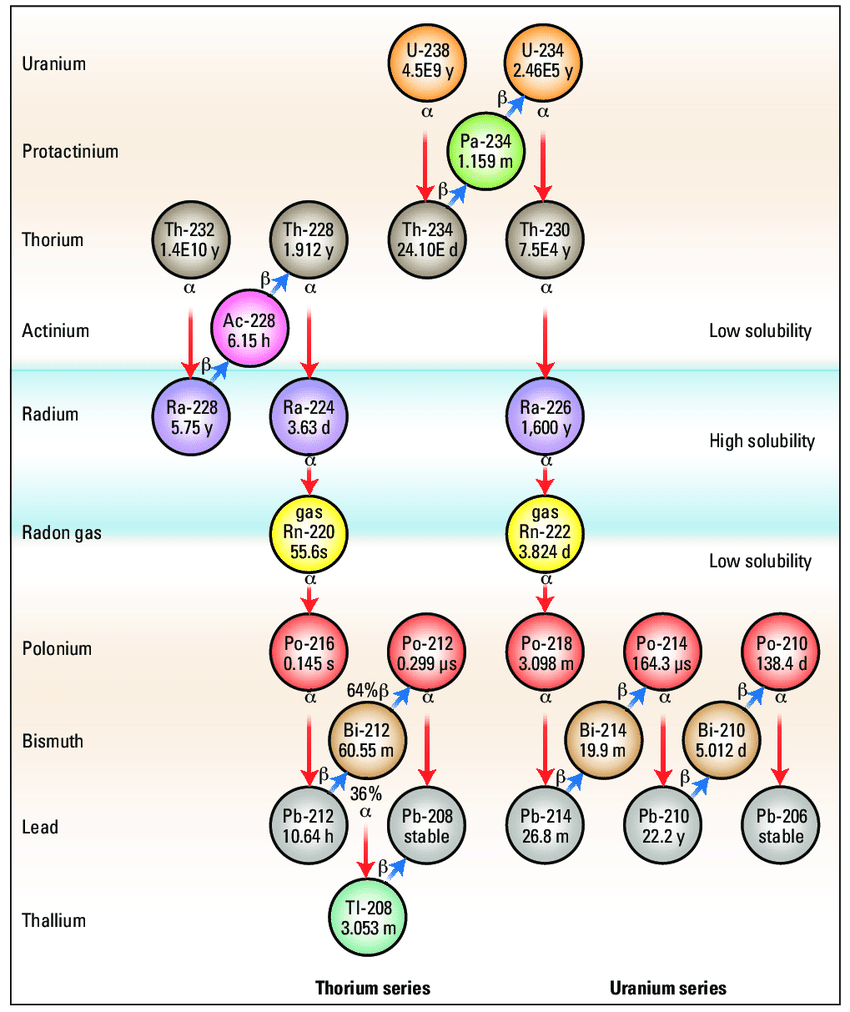
\includegraphics[width=0.8\textwidth]{img/Natural-thorium-and-uranium-decay-chains.png} 
%\vspace*{8pt}
\caption{Natural thorium (left) and uranium (right) decay chains. From \cite{decaychain}.} \label{fig:decaychain}
\end{center}
\end{figure}
%%%%%

Beyond primordial activity, the action of cosmic rays on detector targets and materials may also activate isotopes that would otherwise be stable. Cosmogenic activation of materials may occur both on the surface, during production, transportation or storage, or even underground, during detector operations. While activation on the surface is mostly due to the flux of cosmic-ray neutrons reaching sea level, the one underground is due to cosmic-ray muons\footnote{A depth of a few tens of meter water equivalent (m.w.e.) are sufficient to suppress the flux of cosmic-ray nucleons.}. In the case of underground activation, cosmic-ray muon interactions can produce nuclear breakup ("spallation"), producing a cascade of fast neutrons and electromagnetic showers as a result. The neutrons eventually thermalize and get captured by other nuclei in/near the detector active volume. The resulting neutron-rich nuclei may be unstable, eventually suffering $\beta$ decay, producing both electrons and gamma-rays. This detector activity may be both prompt ($\lesssim$1~ms time delay) or delayed compared to the original muon interaction.

At the depths of underground laboratories, the other only surviving radiation beyond cosmic-ray muons are neutrinos. Very massive detectors, such as liquid-scintillator calorimeters, suffer from an irreducible external background: the solar neutrino flux. Solar neutrinos may elastically scatter off electrons in the detector medium to create energy deposits in the \bbonu\ energy region of interest.

%%%%%%%%%%%%%%%%%%%%%%%%%%%%%%%%%%%%%%%%%%%%%%%%%%%%%%%%%%%%%%%%%%%%%%%%%

\subsection{Sensitivity of a neutrinoless double beta decay experiment} \label{subsec:sensitivitydefinition}

All \bbonu\ experiments have to deal with non-negligible backgrounds, an only partially efficient \bbonu\ event selection, and more or less difficulties to extrapolate their detection technique to large masses. It is instructive, however, to imagine an ideal, background-free, experiment. If such an experiment, after running for an exposure $\Mbb\cdot t$, observes no events, it would report an upper limit in the \bbonu\ decay rate $(\Tonu)^{-1}$, or possibly in the more relevant physical parameter \mbb:
%
\begin{equation}
\mbb = K_{1} \sqrt{\frac{1}{\varepsilon\cdot \Mbb \cdot t}}, \label{eq:mbbx4}
\end{equation}
%
where $K_{1}$ is a constant that depends only on the isotope type, and on the details of the statistical method (and the confidence level) chosen to report such limit. In particular, neglecting factors of order unity, $K_{1}$ is given by:
%
\begin{equation}
K_{1} \simeq \sqrt{\frac{W_{\bb}}{N_A}\cdot \frac{1}{G^{0\nu}\lvert M^{0\nu}\rvert^2}}. \label{eq:k1}
\end{equation}
%
Equations~(\ref{eq:mbbx4}) and \ref{eq:k1} follow directly from eqs.~(\ref{eq:Tonu}) and (\ref{eq:Nbb}), see \cite{Gomez-Cadenas:2010zcc} for details.

Let us now consider the sensitivity in the case of an experiment with background. In the large background approximation, the sensitivity as a function of the background rate $b$ follows the classical limit: $\mathcal{S}(b) \propto \sqrt{b}$, where $b$ is the mean predicted background level. In this limit, the \mbb\ sensitivity can be written as
%
\begin{equation}
\mbb =K_{2} \sqrt{\frac{b^{1/2}}{\varepsilon\cdot \Mbb \cdot t}} 
\label{eq:mbbx1}
\end{equation}
%
where $K_{2}\simeq K_1$ is, again, a constant depending on the isotope (see eq.~\ref{eq:k1}). If the background $b$ is proportional to the exposure $\Mbb \cdot t$ and to an energy window $\Delta E$ around \Qbb :
\begin{equation}
b = c\cdot \Mbb \cdot t\cdot \Delta E
\label{eq:mbbx2}
\end{equation}
%
with the background rate $c$ expressed in \ckkbby, then:
%
\begin{equation}
\mbb = K_2  \ \sqrt{1/\varepsilon} \ \Big(\frac{c\cdot \Delta E}{\Mbb \cdot t}\Big)^{1/4} \label{eq:mbbx3}
\end{equation}
%

In short, the background limits dramatically the sensitivity of a double beta decay experiment, improving only as $(\Mbb \cdot t)^{-1/4}$ instead of the $(\Mbb \cdot t)^{-1/2}$ expected in the background-free case.

Two aspects of eq.~(\ref{eq:mbbx2}), and in particular of our definition of the background rate $c$, deserve further clarification. First, for a given background level $b$, the background rate $c$ will in general depend on the choice of the energy window $\Delta E$, the latter quantity being typically of the order of the FWHM energy resolution of the experiment. This is the case if the background energy spectrum around \Qbb\ is not flat. Similarly, the background rate $c$ will in general depend on the mass \Mbb\ of the \bb\ emitting material considered. This is the case for backgrounds that are not uniformly distributed within the active mass, such as surface contaminations of materials or backgrounds that are of external origin. As already assumed in deriving eq.~(\ref{eq:mbbx3}), all background rate values are relative to the total mass \Mbb\ appearing in the signal count rate computation of eq.~(\ref{eq:Nbb}). 

In the following, we discuss the various ingredients affecting the sensitivity of \bbonu\ experiments.

%%%%%%%%%%%%%%%%%%%%%%%%%%%%%%%%%%%%%%%%%%%%%%%%%%%%%%%%%%%%%%%%%%%%%%%%%%%

\subsection{Choice of the double beta isotope} \label{subsec:isotope}
In nature, 35 naturally-occurring isotopes are \bb\ emitters, but physics and practical considerations dictate that only a few are suitable for \bbonu\ searches.

An ideal \bb\ isotope would: i) maximize the \bbonu\ signal; ii) minimize the contamination of the \bbtnu\ decay; and iii) minimize the impact of radioactive backgrounds. 

Condition i) requires 
%
%Let us start with considerations about the most favorable \bbonu\ phase space factors and nuclear matrix elements. We are interested in the isotopes that provide the highest \bbonu\ rate for the same \mbb\ mass, or, in other words, those that minimize the constants $K_1$ and/or $K_2$ appearing in eqs.~(\ref{eq:mbbx4}) and (\ref{eq:mbbx1}), respectively. As can be seen from eq.~\ref{eq:k1}, this requirement is equivalent to 
%
maximizing the product $G^{0\nu}\cdot\lvert M^{0\nu}\rvert^2/W_{\beta\beta}$ (see eq.~(\ref{eq:mbbx4})). Since $G^{0\nu}(Q,Z)$ varies as $Q_{\beta\beta}^5$ \cite{Vogel:2008sx}, isotopes with large $Q$-values are strongly favored. For this reason, only isotopes with $Q_{\beta\beta}>2$ MeV are usually considered for \bbonu\ searches. The 11 isotopes satisfying this criterion are shown in fig.~\ref{fig:phase_space}. Of the four isotopes used by current experiments and being considered for the next generation (\Ge{76}, \Xe{136}, \Tl{130}, and \Mo{100}),
\Ge{76}, has the less favorable phase space factor (but the lowest $W_{\beta\beta}$ ) while the phase space factor of the other three are rather similar. Unfortunately, the two isotopes with
%The isotopes with the 
the most favorable phase space factors (${\rm ^{150}Nd}$ and ${\rm ^{48}Ca}$), are disfavoured for practical reasons (e.g, isotopic abundance, and enrichment feasibility).  

Fig.~ \ref{fig:NME_full} shows that the values of nuclear matrix elements are rather similar for most isotopes (with the exception of \Ca{48}), and in fact, the uncertainty associated with the predictions of the different models is much large than the variations between isotopes for a given set of NMEs. The net result is that the four isotopes currently in use for \bbonu\ searches would yield a similar sensitivity (differing in no more than a factor two) in an ideal experiment, as illustrated in fig.~\ref{fig:SensiIdeal}.
%Considering the relevant product of the phase space factor times the nuclear matrix element squared over the molar mass for the \bb\ isotopes currently being used in major experiments, we find variations of about a factor of 2 in \mbb\ sensitivity depending on the isotope and for an ideal experiment, as can be seen in fig.~\ref{fig:SensiIdeal} [REPETIR PARA GE, XE, TL, MO ONLY]. 
%From this figure, and from phase space factor and nuclear matrix element considerations alone, we would conclude that \Se{82}, \Te{130} and \Nd{150} would be preferable to \Ge{76}. On the other hand, the molar mass term appearing in eq.~\ref{eq:k1} plays in favor of relatively light isotopes, such as \Ge{76} and \Se{82}. For example, for the same \bb\ isotope mass, a \Ge{76}-based detector contains almost twice as many \b\ nuclides as a \Nd{150}-based detector. Other factors, too, enter in the isotope choice, as discussed below.
 
%%%%%
\begin{figure}[t!b!]
\begin{center}
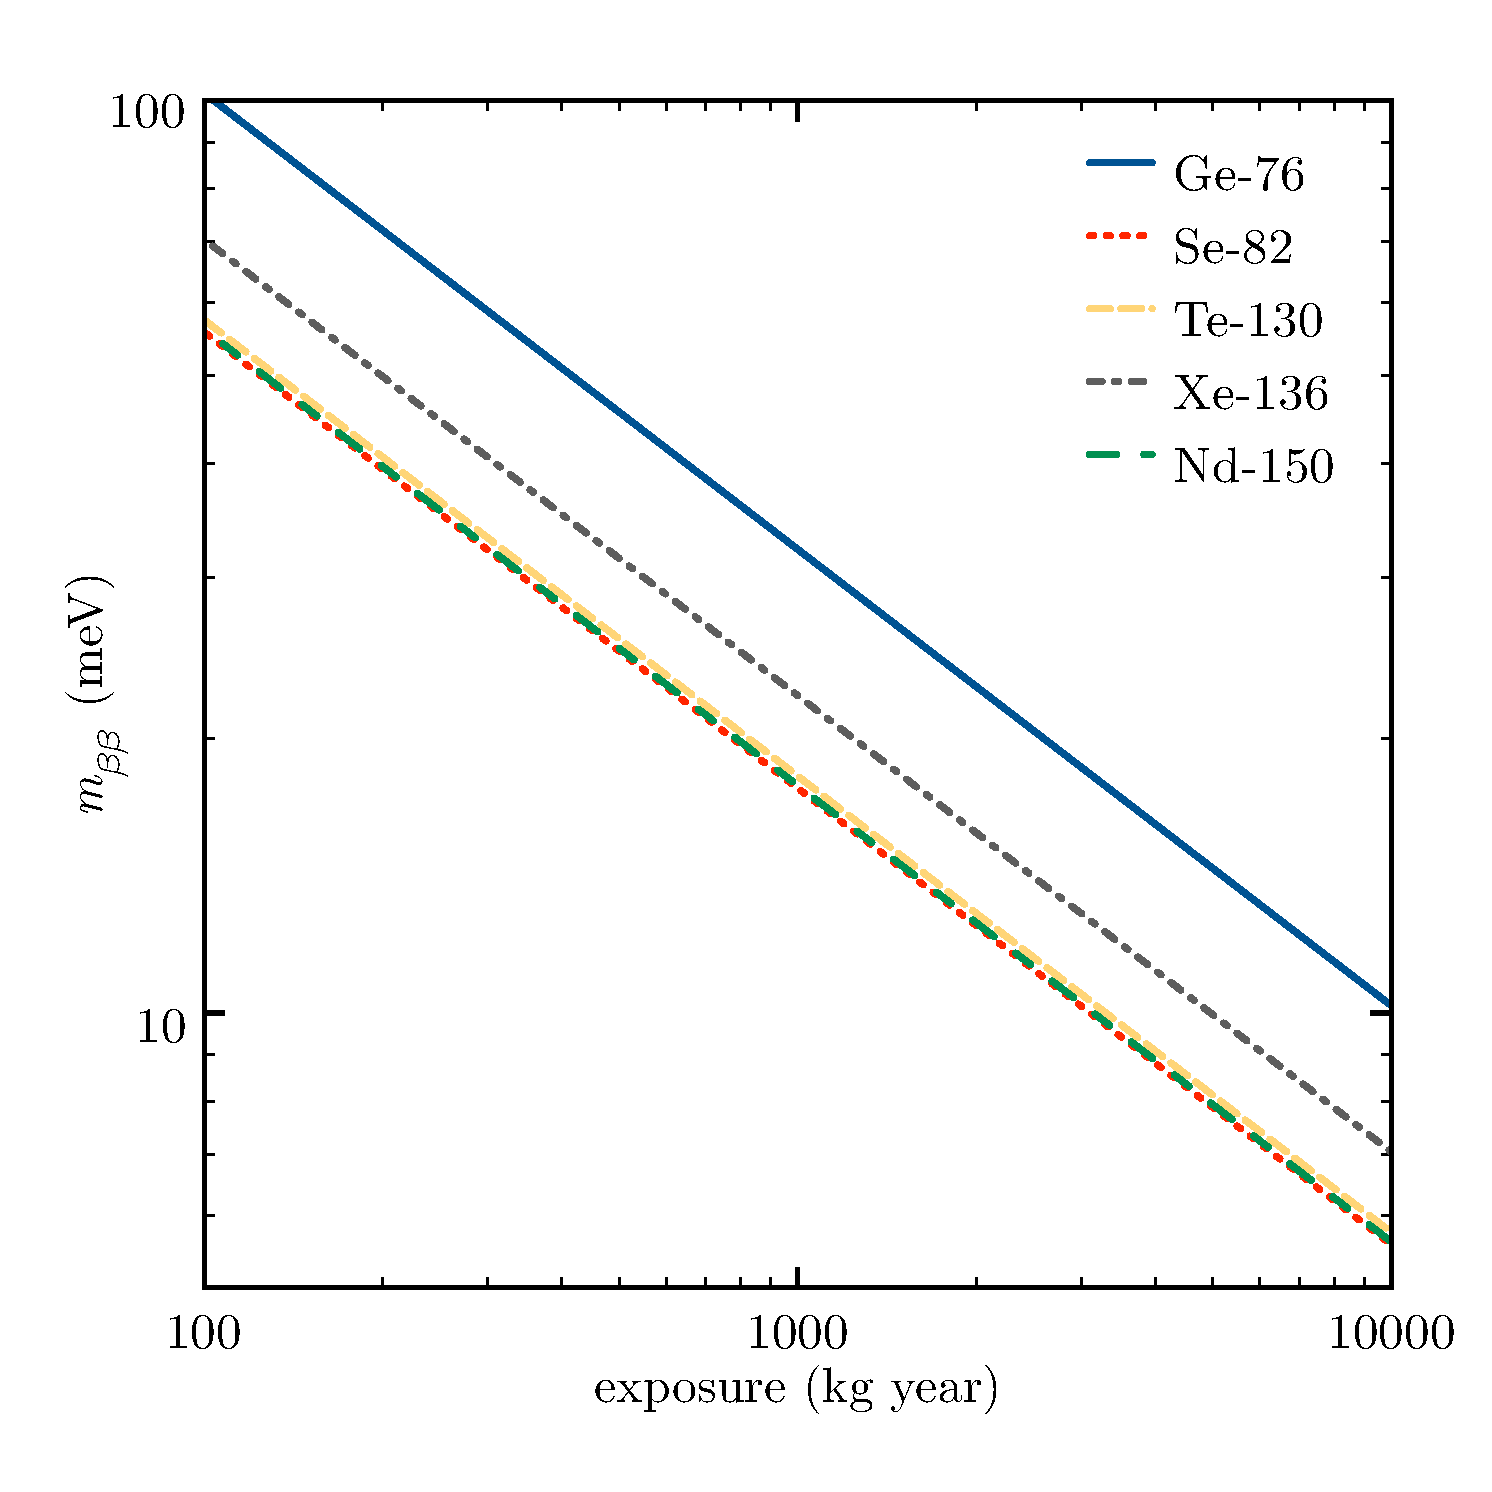
\includegraphics[width=0.65\textwidth]{img/isotopes_sensi.eps}
\end{center}
\caption{Sensitivity of ideal experiments at 90\% CL for different \bb\ isotopes. Since the yields are very similar, the sensitivities of \Se{82}, \Te{130} and \Nd{150} overlap . From reference \cite{Gomez-Cadenas:2010zcc}. TODO: REPEAT FIGURE ADDING MO-100, REMOVING SE-82 AND ND-150} \label{fig:SensiIdeal}	
\end{figure}
%%%%%

Condition iii) also requires choosing a \bb\ isotope with a high $Q_{\beta\beta}$ value. Backgrounds to \bbonu\ searches from natural radioactivity (see fig.~\ref{fig:decaychain}) populate the energy region below $\sim$3 MeV. This makes \Mo{100} which has a Q-value of 3034~keV, a very attractive candidate for \bbonu\ searches, and indeed it has been chosen as target by the future CUPID experiment. On the other hand, condition ii) requires an isotope with a \bbtnu\ mode as slow as possible. The best choice in this case would be \Xe{136} (the choice of EXO-200, kamLAND-Zen, NEXT, and the future nEXO experiment), which has a lifetime in excess of $10^21$~year. Instead, \Mo{100}\ has a lifetime two orders of magnitude faster ($\sim 10^21$~year), and would be disfavoured from this point of view. Conversely, experiments based in \Xe{136} have to deal with two important sources of background located very near the \Qbb\ of \Xe{136} ($\sim 2.5$ MeV), namely, 
\Bi{214} (which emits a gamma that has a photoelectric peak at $\sim 2.4$ MeV), and \Tl{208} (which emits a gamma that has a photoelectric peak at $\sim 2.6$ MeV). The conclusion is that no ideal \bbonu\ isotope exists, and the choices of the different experiments imply alway a number of tradeoffs. 
%As the energy resolution degrades, the experiments are affected by \bbtnu\ backgrounds in a more or less pronounced way, depending on the isotope.  This is true unless the energy resolution of the experiment is truly excellent, in which case even relatively fast \bbtnu\ modes do not constitute a serious background to \bbonu\ searches. This is illustrated in fig.~\ref{fig:twonubgr}. In this figure, the \mbb\ sensitivity at 90\% CL is shown for ideal experiments using five different isotopes as a function of FWHM energy resolution. The experiments, each assumed to use 100 \kgbb\ of \bb\ emitter mass and to run for five years, are ideal in the sense of having perfect \bbonu\ efficiency and of being affected only by \bbtnu\ backgrounds. As fig.~\ref{fig:twonubgr} illustrates, and as far as the \bbtnu\ background is concerned and for the same moderate energy resolution (say, 5-10\% FWHM), \Xe{136} is to be preferred over \Se{82} and \Nd{150}, thanks to its much longer \bbtnu\ half-life (see tab.~\ref{tab:bb2nu_exp}). TODO: MENTION \Te{130} HERE. For experiments featuring excellent energy resolution, say $<2\%$ FWHM, all experiments would operate in a essentially \bbtnu\ background-free regime, for the assumed 500 \kgbb$\cdot$yr exposure. This is typically the case of \Ge{76}, \Mo{100} and some \Te{130} experiments, see sect.~\ref{subsec:energyresolution}.. In practice, however, other backgrounds are always present, typically creating a continuum through the region of interest, and a better resolution improves the experimental sensitivity even in the $<2\%$ FWHM energy resolution range.
%%%%%
%\begin{figure}[t!b!]
%\begin{center}
%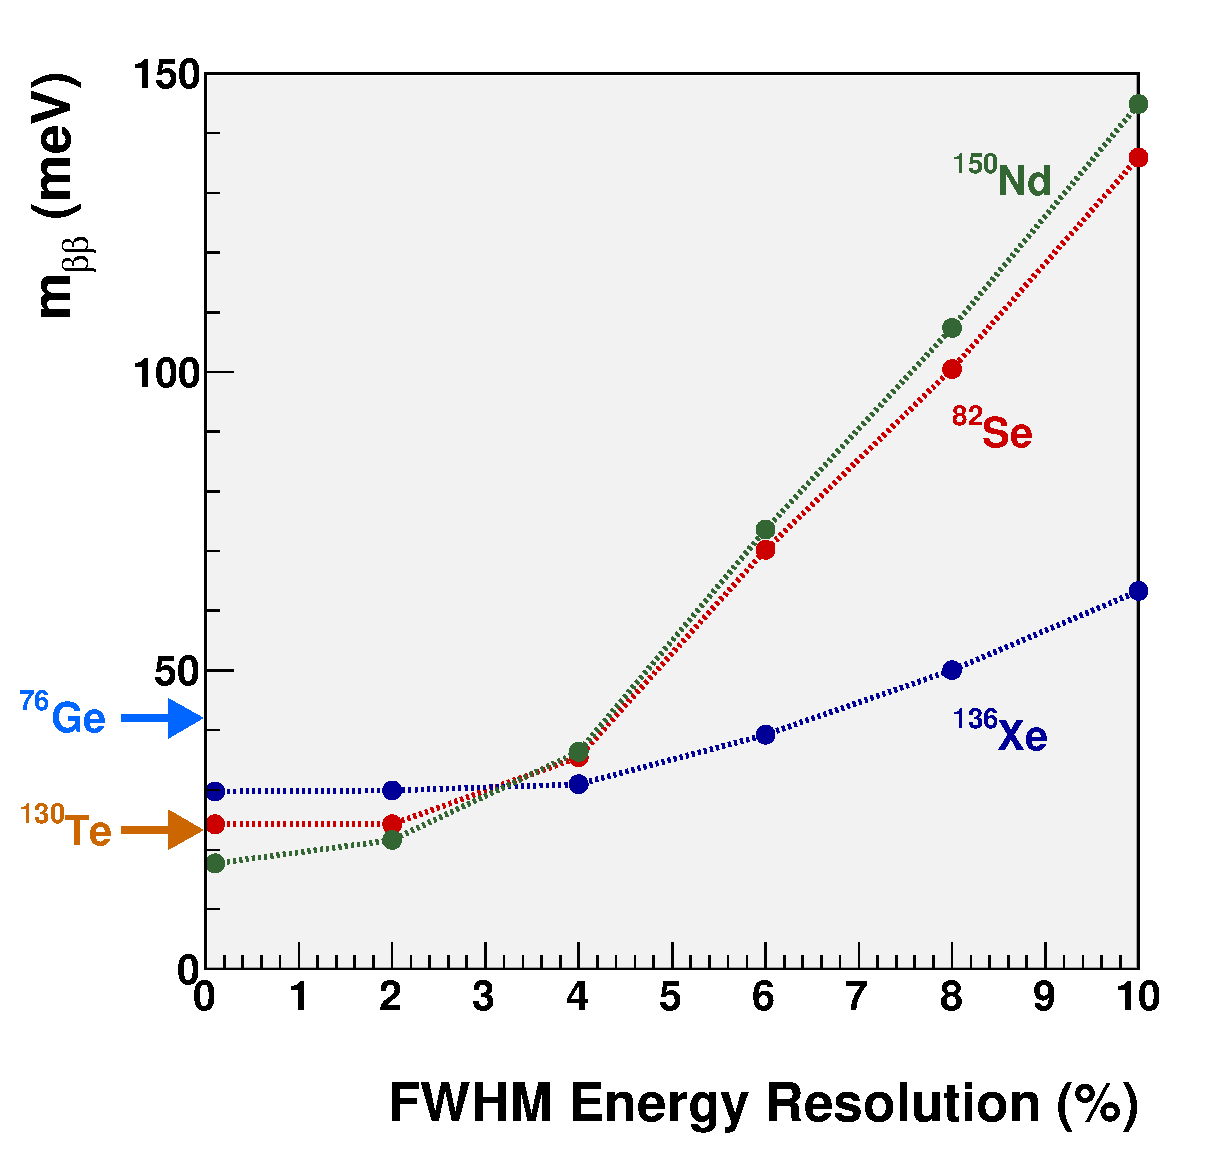
\includegraphics[width=0.65\textwidth]{img/mbbversusenergyres.eps}
%\end{center}
%\caption{\label{fig:twonubgr}Sensitivity to \mbb\ at 90\% CL as a function of FWHM energy resolution, for ideal experiments using five different isotopes, each with 100 \kgbb\ of \bb\ emitter mass and 5 years of data-taking. The experiments are assumed to have perfect efficiency and to be affected only by \bbtnu\ backgrounds. In practice, experiments using \Ge{76} and \Te{130} always feature an excellent energy resolution and are therefore not affected by \bbtnu\ backgrounds, hence only the background-free sensitivity limit is shown in those cases, with an arrow. TODO: REPEAT ADDING MO-100, AND REMOVING SE-82 AND ND-150? TE-130 SHOULD INCLUDE POOR RESOLUTION CASE, THINKING IN SNO+.}  
%\end{figure}
%%%%%

%Finally, another factor entering in the \bb\ isotope choice has to do with how well understood the nuclear physics for that isotope is. As we have seen in sect.~\ref{sec:nme}, the calculation of nuclear matrix elements is a very complicated task. In sect.~\ref{subsec:nme_current}, we have made an attempt at quantifying the uncertainties in the NMEs for various isotopes. Our conclusion is that no \emph{magic isotope} exists, and uncertainties in the 20--30\% range (according to our evaluation) exist for the five isotopes we have considered, \Ge{76}, \Se{82}, \Te{130}, \Xe{136} and \Nd{150}. TODO: UPDATE WITH UNCERTAINTIES FROM FOUR ISOTOPES ONLY: GE-76, MO-100, TE-130, XE-136.  


%%%%%%%%%%%%%%%%%%%%%%%%%%%%%%%%%%%%%%%%%%%%%%%%%%%%%%%%%%%%%%%%%%%%%%%%%%%

\subsection{Isotope mass} \label{subsec:isotope_mass}

As explained above, large masses of \bb\ isotope are needed to explore the expected half-lives. The current generation of double beta decay experiments use masses of the order of 100 kg. New-generation experiments will range from a few hundred kilograms to a few tons, depending on the proposal. Unfortunately, the \bb\ isotopes are not always abundant in nature, often requiring enrichment in order to obtain large, concentrated masses.

The "economy of scale" of large monolithic detectors, such as isotope-loaded liquid scintillators or xenon TPCs, offers a clear advantage for amassing large quantities of \bb\ isotope. Modular approaches where many detector units (eg, crystals) share a common shielding/cryogenic infrastructure are a viable alternative. Let us now examine a few advantageous \bb\ isotopes, as far as mass is concerned.

The current dedicated \bbonu\ experiment employing the largest amount of \bb\ isotope is a \Xe{136}-based one. The KamLAND-Zen 800 experiment uses xenon-loaded liquid scintillator contained in a spherical inner balloon. The amount of enriched xenon dissolved in the scintillator is 745~kg. Considering the (90.85$\pm$0.13)\% \Xe{136} isotopic abundance measured for the enriched xenon, this corresponds to 677~\kgbb\ of \Xe{136} \cite{KamLAND-Zen:2022tow}. There are two reasons that make \Xe{136} a popular choice for massive \bbonu\ experiments. First, its cost is relatively low, and world supply still sufficient for current \bbonu\ demands. The current xenon production is about 100 tons/yr, as a by-product of oxygen extraction from the air for the steel industry. Possible alternative techniques to increase this value are being explored \cite{Avasthi:2021lgy}. The second reason is that isotope enrichment for \Xe{136}, typically based on centrifuge separation methods, is relatively easy and, therefore, cheap. Starting from a 8.9\% isotopic abundance in natural xenon, $\simeq$90\% \Xe{136} isotopic enrichment is typical for \bbonu\ experiments. Beyond xenon-loaded scintillators, xenon TPCs (particularly cryogenic detectors with xenon in its compact, liquid, phase) also represent an excellent solution for large detectors. Dedicated \bbonu\ experiments typically use enriched xenon with $\simeq$90\% enrichment. Realistic proposals for such tonne-scale, or even multi-tonne-scale, experiments exist (see sect.~\ref{subsec:XeTPCs}). Very massive and low-background TPCs filled with natural xenon, primarily developed for direct dark matter searches, also allow for potentially sensitive \bbonu\ searches. One example is the onngoing LUX-ZEPLIN (LZ) experiment, containing about 500~\kgbb\ of \Xe{136} within its 5.6 ton fiducial volume \cite{LZ:2019qdm}.

Liquid scintillator proposals permit in principle to reach large \bbonu\ isotope masses with other isotopes as well, particularly \Te{130}. Tellurium world production is estimated to be $\simeq$500 tons/yr. Tellurium has the advantage of having a high, 34\%, isotopic abundance of the \bb\ emitter \Te{130}. Therefore, the need of isotopic enrichment is typically not considered for \Te{130}-based experiments, greatly reducing costs. Methods for loading \Te{130} into organic liquid scintillators have been developed, particularly in the context of the SNO+ Collaboration. Loading levels up to $\mathcal{O}$(1\%) \Te{130} by weight may be possible in large detetors. Light levels were measured to be reduced compared to unloaded scintillators, but still acceptable. Stability of the loading has been demonstrated on the timescale of years. Water-based liquid scintillators may also be loaded with similar percentages of \Te{130}. Thus, several tons of \Te{130} may be loaded in large liquid scintillator detectors.

High-resolution crystals, that is germanium diodes and bolometers, are compact and modular detectors. They might also be scalable to large masses. The raw \bb\ materials used in this case are available in large supplies, and do not constitute a practical limitation toward massive \bbonu\ experiments. A more challenging scalability aspect is the crystal growth process necessary to fabricate large, kg-scale, crystals of high purity.   

The LEGEND-200 experiment has started taking physics data in 2023. With about 100 high-purity germanium detectors of 0.5--4~kg mass and 86--91\% \Ge{76} enrichment each, a total of about 170~\kgbb\ of \Ge{76} is used. LEGEND-200 has deployed the enriched detectors from the previous GERDA and the Majorana Demonstrator experiments, together with newly-produced inverted-coaxial point-contact (ICPC) detectors, in an upgraded GERDA infrastructure at LNGS. A second phase with 5 times more \Ge{76} mass, LEGEND-1000, is being planned.

The CUORE experiment is searching for the \bbonu\ of \Te{130} with an array of 988 bolometers since 2017. Each bolometer consists of a 750~g $^{nat}$TeO$_2$ crystal, for a total TeO$_2$ mass of over 742 kg, which corresponds to 206~\kgbb\ of \Te{130} \cite{CUORE:2021mvw}. Beyond scalability, bolometers also offer isotopic flexibility. The CUPID-Mo demonstrator \cite{Augier:2022znx} searched for \Mo{100} \bbonu\ with twenty enriched Li$_2$$^{100}$MoO$_4$ (LMO) scintillating calorimeters, each with a mass of about 210~g. Considering the $\simeq$97\% \Mo{100} enrichment, about 2.3~\kgbb\ of \Mo{100} was employed in CUPID-Mo. CUPID is a proposed successor experiment of CUORE based on the CUPID-Mo technology, which plans to use about 250~\kgbb\ of \Mo{100} \cite{CUPID:2019imh}.


%%%%%%%%%%%%%%%%%%%%%%%%%%%%%%%%%%%%%%%%%%%%%%%%%%%%%%%%%%%%%%%%%%%%%%%%%%%

\subsection{Energy resolution} \label{subsec:energyresolution}
%
Together with a large isotope mass, good energy resolution is a necessary (but not sufficient!) requirement for the \emph{ultimate} \bbonu\ experiment. It is the only protection against the intrinsic \bbtnu\ background, and improves the signal-to-noise ratio in the region of interest around \Qbb. 

The detectors for \bb\ searches that have achieved the best energy resolution so far are the \emph{germanium diodes} and the \emph{bolometers}. 

In germanium detectors the energy is measured via ionization (creation of electron-hole pairs in the semiconductor). The exposure-averaged FWHM energy resolution of the Ge detectors used in the final GERDA Phase II result was only 3.3$\pm$0.4~keV \cite{GERDA:2020xhi}. Considering that the \Qbb\ value in \Ge{76} is 2039~keV, this corresponds to a relative energy resolution of 0.16\% (FWHM). In particular, the large ICPC-type detectors constituting the bulk of the LEGEND-200 detectors featured an even better energy resolution of 2.9$\pm$0.1~keV (FWHM). 

In bolometers the energy is measured by detecting a temperature rise in crystals with very small specific heat. Several bolometric crystals have been proposed and tested for \bb\ searches, such as tellurite (TeO$_{2}$), lithium molybdate (LMO, Li$_2$$^{100}$MoO$_4$) and zinc selenide (ZnSe). For these three technologies, FWHM energy resolutions at the Q-values of the corresponding \bb\ emitters were measured to be: 7.8$\pm$0.5 \cite{CUORE:2021mvw}, 7.6$\pm$0.7 \cite{CUPID:2020aow} and 21.8$\pm$0.3 keV \cite{CUPID:2022puj}, respectively. TeO$_{2}$ and LMO detectors thus feature similar resolution performance among them based on the heat measurement, and superior to the ZnSe one. However, as we will see in the following (sect.~\ref{subsec:bgr_mitigation}), LMO detectors offer an advantage over TeO$_{2}$ ones, as they provide an additional scintillation light signal.



 
%%%%%%%%%%%%%%%%%%%%%%%%%%%%%%%%%%%%%%%%%%%%%%%%%%%%%%%%%%%%%%%%%%%%%%%%%%

\subsection{Background mitigation (other than energy resolution)} \label{subsec:bgr_mitigation}

Double beta decay experiments are mostly about suppressing the background sources mentioned in Sect.~\ref{subsec:bgr_sources}. As we have seen already, the mere presence of background in the region of interest around \Qbb\ changes the regime of the \mbb\ sensitivity from a $(\Mbb \cdot t)^{-1/2}$ dependence to $(\Mbb \cdot t)^{-1/4}$. In the following, we describe the background mitigation techniques employed by \bbonu\ experiments. These can be separated into {\emph passive} and {\emph active} techniques, depending on whether detector information is used or not.

Starting with passive mitigation techniques, the use of detector materials with extremely low amounts of radioactive impurities is key. Selection, manufacturing, cleaning and installation of detector materials has to be conducted with extreme care in all \bbonu\ experiments, relying on radio-pure protocols at all times. Material selection is based on extensive radio-purity assays of all detector materials, using both gamma spectroscopy and mass spectrometry techniques. Cleaning of detector components is necessary to remove surface contaminants, such as dust or lubricants from the manufacturing processes. Cleaning is carried out in detergent and acidic solutions, sometimes using ultrasonic techniques. Dedicated manufacturing processes are used to avoid contamination. Detector installation occurs in clean-room conditions. The most stringent radio-purity requirements apply to the detector active target itself, as well as to other massive detector components (e.g., shielding parts) in close proximity to it. The new-generation experiments are being fabricated from amazingly radio-pure components, some with specific activities as low as 1 $\mu$Bq/kg or less. Specific activities that are that low require \Th{232} and \U{238} impurities in the bulk materials that are below the part per trillion (ppt) level in mass, $<10^{-12}$~g/g. Ultra-pure detector material examples include organic scintillator and xenon fluids through closed-loop re-circulation and purification systems, 2,000 year old Roman shielding lead, and fabrication of ultra-pure shielding copper via electroforming techniques.

Beyond primordial activity from contaminants in the natural decay chains, production inside detector materials of radioactive nuclides by cosmic-rays may also occur. Cosmogenic activation is, of course, more severe on surface. Therefore, for experiments using materials that can get activated (like germanium-based experiments), underground fabrication and storage of the detector components is essential.

Radon gas, particularly \Rn{222}, is an intermediate by-product of the natural decay chains, that also needs to be suppressed inside and near \bbonu\ experiments. Being gaseous, radon does not stay trapped within detector components and may infiltrate inside detector sensitive regions, hence requiring a separate mitigation strategy. Also, radon daughters tend to be electrically charged and stick to surfaces. Concerning airborne radon, most deep underground laboratories have radon abatement systems capable of suppressing the radon concentration in the air by several orders of magnitude, down to 1 mBq/m$^3$ concentrations, providing effectively radon-free air in the vicinity of the detectors. The flushing of pure nitrogen gas is an equally effective, although more expensive, alternative to provide a radon-free environment. The radon concentration in the air is monitored in real-time at underground locations. Radon may also diffuse inside fluid-based (liquid or gaseous) \bbonu\ detectors, typically via emanation from detector materials. Active filtration systems (radon traps) may be used to mitigate this internal radon component.

Concerning external backgrounds originated outside the detectors, the techniques to passively mitigate them involve placing the experiments at deep underground laboratories, and by enclosing them into shielding systems. 

Deep underground laboratories are research infrastructures with an overburden typically larger than 1000 meters water equivalent (m.w.e.). In general, the depth requirement for a \bbonu\ experiment varies according to the detector technology. A very efficient shielding and additional detection signatures such as topological information can compensate the benefits of a very deep location. Figure \ref{fig:underground_facilities} shows the laboratory depth and size of several underground facilities currently available to host physics experiments around the world. In addition to depth, other important factors characterizing the underground sites include the size of the excavated halls available for science, and the services provided to the experiments. The size is an important factor to take into account especially for experimental proposals at the ton-scale and beyond, given that some of them need large volumes. The most relevant deep underground laboratories for current and future \bbonu\ experiments, listed in order of decreasing depth, are at the moment: the China Jinping Underground Laboratory (CJPL, China), SNOLAB (Canada), the Gran Sasso National Laboratory (LNGS, Italy), the Sanford Underground Research Facility (SURF, USA), the Kamioka Observatory (Japan) and the Canfranc Underground Laboratory (LSC, Spain). For a recent review of the currently available underground facilities around the world, see reference \cite{Ianni:2023fvs}. 

%%%%%
\begin{figure}[t!b!]
\begin{center}
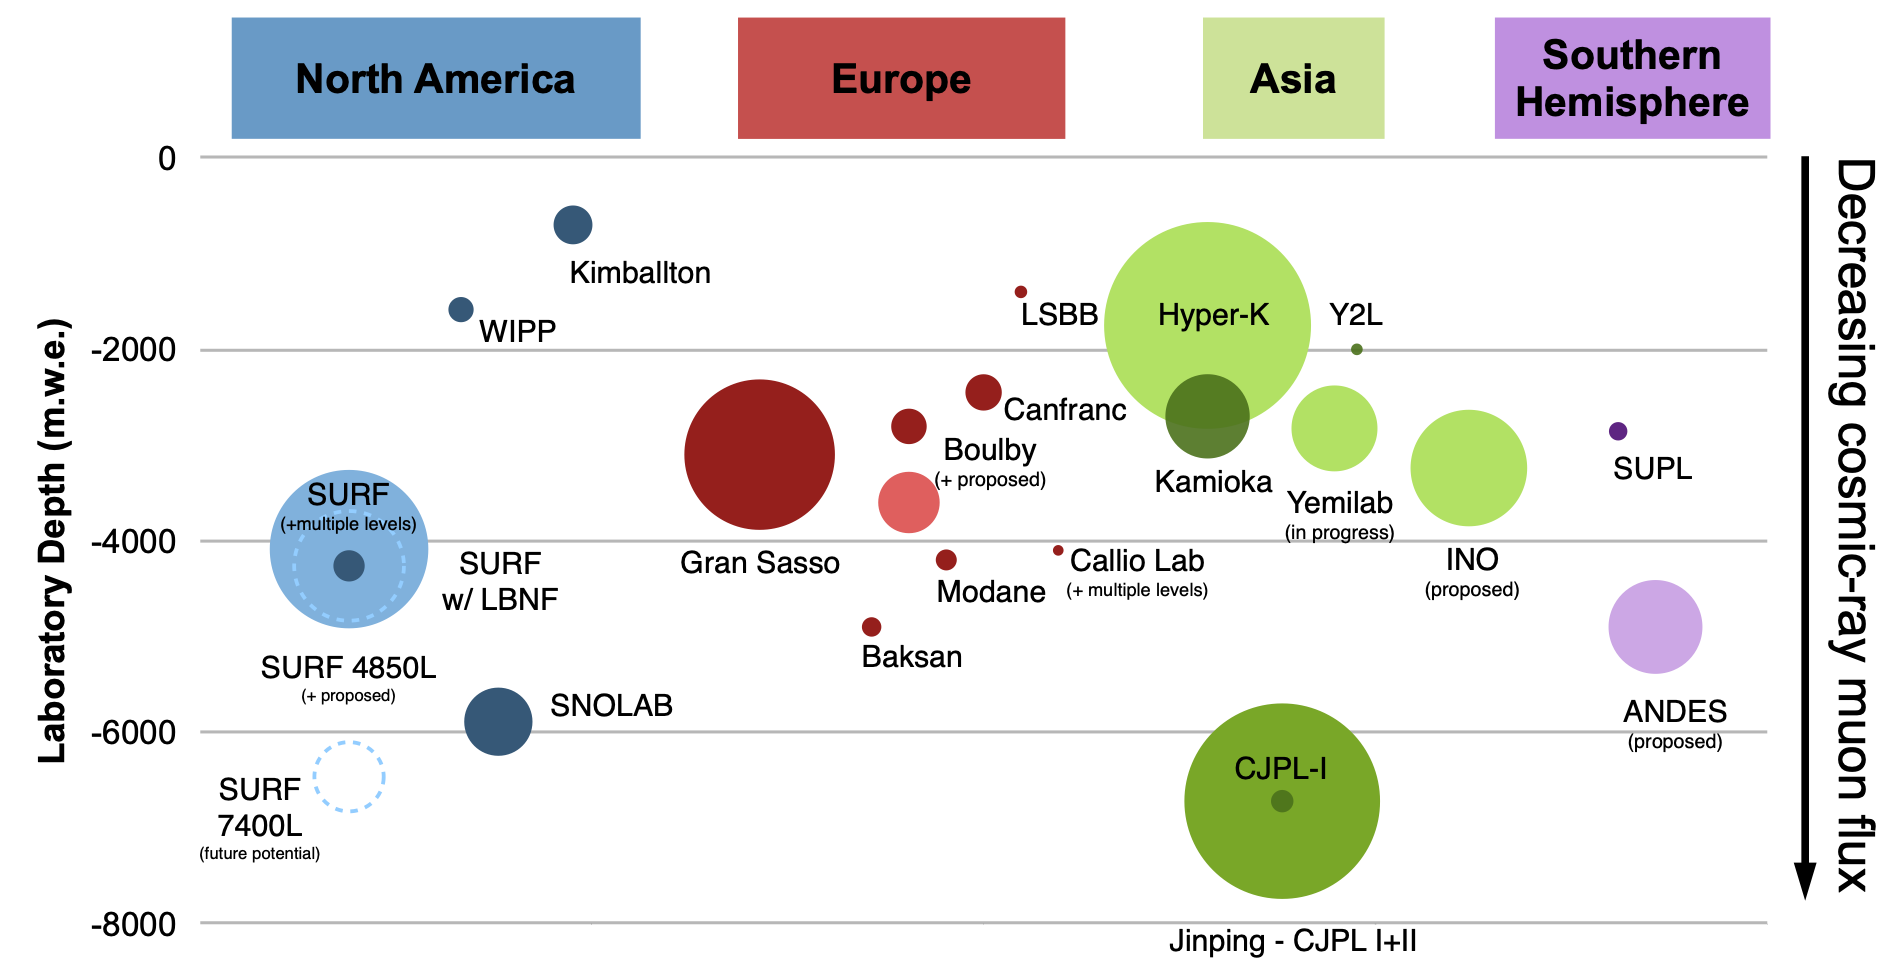
\includegraphics[width=\textwidth]{img/UndergroundFacilities.png}
%\vspace*{8pt}
\caption{\label{fig:underground_facilities}Overview of underground facilities located around the world. The size (volume of science space) and effective shielding depth (total muon flux) are shown. Some muon flux values are estimated using a recent parameterization \cite{JNE:2020bwn}. Figure from \cite{Baudis:2022pzb,Heise:2022iaf}.}
\end{center}
\end{figure}
%%%%%

Shielding systems surrounding the detectors are another very effective technique to passively suppress external backgrounds. As such, they are used ubiquitously in \bbonu\ experiments. In the design of a shielding system against external backgrounds, a \emph{graded shielding} principle is followed: the thickness of a shield component does not need to reduce the flux below the contribution of the next inner component, with the innermost shield component selected to be the radiopurest.

Despite their sizable penetrating power, external neutrons from cosmic-ray interactions and from $(\alpha$,n) reactions can be shielded with layers of hydrogenous material. On the other hand, the external $\gamma$-ray flux produced by radioactive decays in the rock of the underground cavern can be suppressed via dense, high $Z$, radiopure materials such as lead and copper. 

Liquid shields in the form of water tanks, LAr-filled cryostats or liquid scntillator buffers, are also good option for shielding against neutrons and $\gamma$-rays. Liquid shields have two additional advantages over solid ones: they can be continuously purified, and they may be turned into {\emph active} veto systems. This is possible by instrumenting them as Cherenkov/scintillation light detectors in order to tag the passage of charged particles. Plastic scintillator detectors are also often used as active veto systems against external backgrounds. Such anti-coincidence techniques, between an inner detector containing the \bbonu\ target and outer detectors, constitute a powerful active background mitigation technique. 

Excellent energy resolution is, of course, another powerful active background mitigation technique, and has been discussed already, see Sect.~\ref{subsec:energyresolution}. There are, however, many other active background mitigation techniques beyond veto systems and energy resolution. 

In addition to anti-coincidence requirements in space, delayed coincidences in time are also used to suppress backgrounds. This is the case for sequential radioactive decays with relatively short-lived isotopes. A prime example is \Bi{214}-induced background suppression via the delayed \Po{214} tag, where the \Po{214} $\alpha$ decay has a 164.3~$\mu$s half-life. 

Signal and background events have also different spatial distributions. Signal events are typically distributed uniformly in the detector volume. External backgrounds accumulate on, or enter from, detector surfaces. This is also exploited to suppress backgrounds via detector fiducialization. 

The topological information of the energy deposits in the active volume is also used. Gamma-ray background interactions producing multi-site energy deposits, typically via multi-Compton interactions, may be readily vetoed in segmented or imaging detectors. Pulse shape analysis in individual Ge detectors is an alternative way to identify and suppress multi-site backgrounds. Low density detectors, such as xenon gas TPCs and where MeV-scale particles produce extended tracks, provide even more detailed topological information. In this case, information from the reconstructed $dE/dx$ energy loss profiles along the track can distinguish single-electron background events from double-electron signal events.

Particle identification is another powerful background suppression handle. A notable example is $\alpha/\beta$ discrimination in scintillating bolometers. As the light yield for energy depositions induced by $\alpha$ and $\beta$ particles of the same energy is different, the simultaneous detection of light and heat leads to an effective rejection of the $\alpha$ background. 

Finally, another handle to suppress non-\bbtnu\ backgrounds is \emph{daughter ion tagging} in coincidence with the detection of the two beta electrons. This has been proposed, and is actively being pursued, for both liquid and gas xenon TPC detectors. In this case, the \bbonu\ decay is ${\rm ^{136}Xe}\to {\rm ^{136}Ba^{++}}+2e^-$. In liquid, the \Ba{136}$^{++}$ ion rapidly captures an electron in the charge cloud following a \bb\ event, resulting in \Ba{136}$^{+}$, and barium neutralization may also occur. In the less dense gas environment, no recombination is expected, and the \Ba{136}$^{++}$ doubly-charged state remains stable. Recently, both the nEXO \cite{nEXO:2018nxx} and NEXT \cite{McDonald:2017izm,Rivilla:2020cvm} collaborations made substantial progress in isolating and detecting a lone Ba ion in-situ, via fluorescence imaging techniques. Daughter ion tagging is undoubtedly very challenging from the technical point of view, but the payoff would be huge if the R\&D were to be successful.

The lowest background rates ($c$ term in eq.~\ref{eq:mbbx2}, expressed in terms of background events per unit energy, \bb\ isotope mass and exposure time) in a \bbonu\ experiment so far were achieved by the KamLAND-Zen (see sect.~\ref{subsec:liquid_scint}) and GERDA (sect.~\ref{subsec:hpge}) experiments. Perhaps not surprisingly, given the importance of background suppression in \bbonu\ experiments, these are also the two experiments with the most stringent \bbonu\ half-life upper limits to date, see tab.~\ref{tab:bb0nu_exp}. KamLAND-Zen 800 has achieved a background rate of $1.3\times 10^{-4}$ \ckkbby\ \cite{KamLAND-Zen:2022tow}, thanks to its outstanding radio-purity, shielding and anti-coincidence techniques. On the other hand, GERDA Phase II has achieved $6.0\times 10^{-4}$ \ckkbby\ \cite{GERDA:2020xhi}, thanks to its ultra-pure crystals and pulse shape discrimination techniques. 

Finally, we remark that the relevant background figure of merit, the one appearing in the \mbb\ sensitivity of eq.~\ref{eq:mbbx3}, is given by the product $c\cdot \Delta E$, that is the number of background events per unit time and \bb\ isotope mass in the entire region of interest\footnote{For simplicity, we are assuming here that the energy regiopn of interest around \Qbb\ has a width equal to the FWHM energy resolution, $\Delta E$.}. According to this figure of merit, GERDA Phase II is the current record holder in terms of lowest background conditions, with a $c\cdot \Delta E$ value of 0.002 counts/$(\kgbb\cdot\ensuremath{year})$. Considering that GERDA Phase II has accumulated a total exposure of 90.2 \kgbb$\cdot$year, the mean number of background events expected within \Qbb $\pm$ FWHM/2 was about 0.2, consistent with observations. In other words, GERDA Phase II accomplished its goal of background-free conditions. The goal of the new-generation experiments is typically to reach $10^{-4}$ \ckkbby\ background levels, and sometimes significantly better than that (eg, LEGEND-1000).



%%%%%%%%%%%%%%%%%%%%%%%%%%%%%%%%%%%%%%%%%%%%%%%%%%%%%%%%%%%%%%%%%%%%%%%%%%

\subsection{Detection efficiency} \label{subsec:efficiency}

Neutrinoless double beta decay events are extremely rare, if present at all, thus a high detection efficiency is an important requirement for a \bb\ experiment. Equation~(\ref{eq:mbbx3}) clearly indicates that the detector design should prioritize a high detection efficiency. To obtain the same increase in \mbb\ sensitivity obtained by doubling the efficiency, the mass would have to be increased by a factor of 4, assuming the same background.

In general, the simpler the detection scheme, the higher the detection efficiency. Homogeneous detectors, where the source material is the detection medium, provide in principle higher efficiency than a separate-source approach. This is due to a number of reasons, including geometric acceptance, absorption in the \bb\ source, back-scattering of electrons, and tracking requirements.

Pure calorimetric approaches such as germanium diodes or bolometers tend to have the highest total signal efficiencies, and values in excess of 75\% have been obtained. 

For the CUORE bolometric \bbonu\ search in \Te{130}, the total efficiency is 81.6$\pm$0.2\%, given by the product of the reconstruction, anti-coincidence, pulse shape discrimination and containment efficiencies \cite{CUORE:2021mvw}. The main inefficiency comes from containment requirements, accounting for the energy loss due to geometrical effects as well as bremsstrahlung.

In the case of germanium diodes, the exposure-averaged efficiency in the final GERDA \bbonu\ search was 63.0$\pm$5.6\%, given by the product of electron containment, active volume, liquid argon veto and pulse shape discrimination requirements \cite{GERDA:2020xhi}. For the ICPC-type detectors alone employed in LEGEND-200, the total efficiency increases to 75.2$\pm$2.1\%, thanks to their larger crystal sizes and intrinsically better performance.

Large liquid scintillators may also have relatively high efficiencies. This is especially the case when the \bb\ source is enclosed in a inner balloon surrounded by a scintillator buffer region, as in the KamLAND-Zen experiment. The detector dead-time to tag and reject comsogenic backgrounds (about $\simeq$15\% in \cite{KamLAND-Zen:2022tow}) is a relevant inefficiency, in this case. Depending on the \bbonu\ analysis details, the relatively poor energy and spatial resolutions may also introduce, effectively, additional inefficiencies. For example, about 22\% of the putative \bbonu\ events would fall outside a 350~keV wide energy region of interest around \Qbb\ in \cite{KamLAND-Zen:2022tow}.

Liquid xenon TPCs share the same advantages of the other dense, homogeneous, detectors. However, they use some of the \bb\ mass close to the detector borders effectively for self-shielding, paying it with some efficiency loss.

Some experiments perform particle tracking, such as planar configurations of \bb\ foils separate from detector media, or homogeneous xenon gas TPC. The tracking requirements typically cause a significant efficiency loss. 


%%%%%%%%%%%%%%%%%%%%%%%%%%%%%%%%%%%%%%%%%%%%%%%%%%%%%%%%%%%%%%%%%%%%%%%%%